\documentclass[12pt,letterpaper,oneside,oldfontcommands]{memoir}
\usepackage{lmodern}
\usepackage{amssymb,amsmath}
\usepackage{ifxetex,ifluatex}
\usepackage{fixltx2e} % provides \textsubscript
\ifnum 0\ifxetex 1\fi\ifluatex 1\fi=0 % if pdftex
  \usepackage[T1]{fontenc}
  \usepackage[utf8]{inputenc}
\else % if luatex or xelatex
  \ifxetex
    \usepackage{mathspec}
  \else
    \usepackage{fontspec}
  \fi
  \defaultfontfeatures{Ligatures=TeX,Scale=MatchLowercase}
\fi
% use upquote if available, for straight quotes in verbatim environments
\IfFileExists{upquote.sty}{\usepackage{upquote}}{}
% use microtype if available
\IfFileExists{microtype.sty}{%
\usepackage{microtype}
\UseMicrotypeSet[protrusion]{basicmath} % disable protrusion for tt fonts
}{}
\usepackage[margin=1in]{geometry}
\usepackage{hyperref}
\hypersetup{unicode=true,
            pdftitle={My Predissertation Paper},
            pdfauthor={Tricia Marie McMillan},
            pdfborder={0 0 0},
            breaklinks=true}
\urlstyle{same}  % don't use monospace font for urls
\usepackage{natbib}
\bibliographystyle{apalike}
\usepackage{color}
\usepackage{fancyvrb}
\newcommand{\VerbBar}{|}
\newcommand{\VERB}{\Verb[commandchars=\\\{\}]}
\DefineVerbatimEnvironment{Highlighting}{Verbatim}{commandchars=\\\{\}}
% Add ',fontsize=\small' for more characters per line
\usepackage{framed}
\definecolor{shadecolor}{RGB}{248,248,248}
\newenvironment{Shaded}{\begin{snugshade}}{\end{snugshade}}
\newcommand{\AlertTok}[1]{\textcolor[rgb]{0.94,0.16,0.16}{#1}}
\newcommand{\AnnotationTok}[1]{\textcolor[rgb]{0.56,0.35,0.01}{\textbf{\textit{#1}}}}
\newcommand{\AttributeTok}[1]{\textcolor[rgb]{0.77,0.63,0.00}{#1}}
\newcommand{\BaseNTok}[1]{\textcolor[rgb]{0.00,0.00,0.81}{#1}}
\newcommand{\BuiltInTok}[1]{#1}
\newcommand{\CharTok}[1]{\textcolor[rgb]{0.31,0.60,0.02}{#1}}
\newcommand{\CommentTok}[1]{\textcolor[rgb]{0.56,0.35,0.01}{\textit{#1}}}
\newcommand{\CommentVarTok}[1]{\textcolor[rgb]{0.56,0.35,0.01}{\textbf{\textit{#1}}}}
\newcommand{\ConstantTok}[1]{\textcolor[rgb]{0.00,0.00,0.00}{#1}}
\newcommand{\ControlFlowTok}[1]{\textcolor[rgb]{0.13,0.29,0.53}{\textbf{#1}}}
\newcommand{\DataTypeTok}[1]{\textcolor[rgb]{0.13,0.29,0.53}{#1}}
\newcommand{\DecValTok}[1]{\textcolor[rgb]{0.00,0.00,0.81}{#1}}
\newcommand{\DocumentationTok}[1]{\textcolor[rgb]{0.56,0.35,0.01}{\textbf{\textit{#1}}}}
\newcommand{\ErrorTok}[1]{\textcolor[rgb]{0.64,0.00,0.00}{\textbf{#1}}}
\newcommand{\ExtensionTok}[1]{#1}
\newcommand{\FloatTok}[1]{\textcolor[rgb]{0.00,0.00,0.81}{#1}}
\newcommand{\FunctionTok}[1]{\textcolor[rgb]{0.00,0.00,0.00}{#1}}
\newcommand{\ImportTok}[1]{#1}
\newcommand{\InformationTok}[1]{\textcolor[rgb]{0.56,0.35,0.01}{\textbf{\textit{#1}}}}
\newcommand{\KeywordTok}[1]{\textcolor[rgb]{0.13,0.29,0.53}{\textbf{#1}}}
\newcommand{\NormalTok}[1]{#1}
\newcommand{\OperatorTok}[1]{\textcolor[rgb]{0.81,0.36,0.00}{\textbf{#1}}}
\newcommand{\OtherTok}[1]{\textcolor[rgb]{0.56,0.35,0.01}{#1}}
\newcommand{\PreprocessorTok}[1]{\textcolor[rgb]{0.56,0.35,0.01}{\textit{#1}}}
\newcommand{\RegionMarkerTok}[1]{#1}
\newcommand{\SpecialCharTok}[1]{\textcolor[rgb]{0.00,0.00,0.00}{#1}}
\newcommand{\SpecialStringTok}[1]{\textcolor[rgb]{0.31,0.60,0.02}{#1}}
\newcommand{\StringTok}[1]{\textcolor[rgb]{0.31,0.60,0.02}{#1}}
\newcommand{\VariableTok}[1]{\textcolor[rgb]{0.00,0.00,0.00}{#1}}
\newcommand{\VerbatimStringTok}[1]{\textcolor[rgb]{0.31,0.60,0.02}{#1}}
\newcommand{\WarningTok}[1]{\textcolor[rgb]{0.56,0.35,0.01}{\textbf{\textit{#1}}}}
\usepackage{longtable,booktabs}
\usepackage{graphicx,grffile}
\makeatletter
\def\maxwidth{\ifdim\Gin@nat@width>\linewidth\linewidth\else\Gin@nat@width\fi}
\def\maxheight{\ifdim\Gin@nat@height>\textheight\textheight\else\Gin@nat@height\fi}
\makeatother
% Scale images if necessary, so that they will not overflow the page
% margins by default, and it is still possible to overwrite the defaults
% using explicit options in \includegraphics[width, height, ...]{}
\setkeys{Gin}{width=\maxwidth,height=\maxheight,keepaspectratio}
\IfFileExists{parskip.sty}{%
\usepackage{parskip}
}{% else
\setlength{\parindent}{0pt}
\setlength{\parskip}{6pt plus 2pt minus 1pt}
}
\setlength{\emergencystretch}{3em}  % prevent overfull lines
\providecommand{\tightlist}{%
  \setlength{\itemsep}{0pt}\setlength{\parskip}{0pt}}
\setcounter{secnumdepth}{5}
% Redefines (sub)paragraphs to behave more like sections
\ifx\paragraph\undefined\else
\let\oldparagraph\paragraph
\renewcommand{\paragraph}[1]{\oldparagraph{#1}\mbox{}}
\fi
\ifx\subparagraph\undefined\else
\let\oldsubparagraph\subparagraph
\renewcommand{\subparagraph}[1]{\oldsubparagraph{#1}\mbox{}}
\fi

%%% Use protect on footnotes to avoid problems with footnotes in titles
\let\rmarkdownfootnote\footnote%
\def\footnote{\protect\rmarkdownfootnote}

%%% Change title format to be more compact
\usepackage{titling}

% Create subtitle command for use in maketitle
\newcommand{\subtitle}[1]{
  \posttitle{
    \begin{center}\large#1\end{center}
    }
}

\setlength{\droptitle}{-2em}
  \title{My Predissertation Paper}
  \pretitle{\vspace{\droptitle}\centering\huge}
  \posttitle{\par}
  \author{Tricia Marie McMillan}
  \preauthor{\centering\large\emph}
  \postauthor{\par}
  \predate{\centering\large\emph}
  \postdate{\par}
  \date{2018-04-25}


\usepackage{booktabs}
\usepackage{amsthm}
\usepackage{microtype}
\usepackage{xltxtra}
\usepackage{hyperref}
\usepackage{datetime}
\usepackage{float}
\usepackage{adforn}
\usepackage[table]{xcolor}
\usepackage{fix-cm}


\makeatletter
\def\thm@space@setup{%
  \thm@preskip=8pt plus 2pt minus 4pt
  \thm@postskip=\thm@preskip
}
\makeatother


%%%%%%%%%%%%%%%%%%%%%%%%%%%%%%%%%%%%%%%%%%%%%%%%%%%%%%%%%%%%%%%%%%%%%%%%
% Define colors
%%%%%%%%%%%%%%%%%%%%%%%%%%%%%%%%%%%%%%%%%%%%%%%%%%%%%%%%%%%%%%%%%%%%%%%%

\definecolor{numbercolor}{gray}{0.7}
\definecolor{smartblue}{HTML}{193A6B}



%%%%%%%%%%%%%%%%%%%%%%%%%%%%%%%%%%%%%%%%%%%%%%%%%%%%%%%%%%%%%%%%%%%%%%%%
% Set fonts
%%%%%%%%%%%%%%%%%%%%%%%%%%%%%%%%%%%%%%%%%%%%%%%%%%%%%%%%%%%%%%%%%%%%%%%%

\defaultfontfeatures{Mapping=tex-text}
\newfontfamily{\smallcaps}[RawFeature={c2sc,scmp}]{EB Garamond}
\defaultfontfeatures{Ligatures=TeX}
\setmainfont[Numbers=OldStyle, Contextuals=Alternate, Ligatures={Common}]{EB Garamond}
\setsansfont[Scale=MatchLowercase, BoldFont={Lato Bold}]{Lato Regular}
\setmonofont[Scale=MatchLowercase]{Source Code Pro}



%%%%%%%%%%%%%%%%%%%%%%%%%%%%%%%%%%%%%%%%%%%%%%%%%%%%%%%%%%%%%%%%%%%%%%%%
% Basic page layout
%%%%%%%%%%%%%%%%%%%%%%%%%%%%%%%%%%%%%%%%%%%%%%%%%%%%%%%%%%%%%%%%%%%%%%%%

\usepackage{calc}
\setlrmarginsandblock{1.5in}{1in}{*}
\setulmarginsandblock{1in + \headheight + \headsep}{1in + \footskip}{*}
\DoubleSpacing
\checkandfixthelayout
\setlength\evensidemargin{\oddsidemargin}



%%%%%%%%%%%%%%%%%%%%%%%%%%%%%%%%%%%%%%%%%%%%%%%%%%%%%%%%%%%%%%%%%%%%%%%%
% Some nice chapter headings
%%%%%%%%%%%%%%%%%%%%%%%%%%%%%%%%%%%%%%%%%%%%%%%%%%%%%%%%%%%%%%%%%%%%%%%%

\newif\ifchapternonum
\makechapterstyle{jenor}{
  \renewcommand\printchaptername{}
  \renewcommand\printchapternum{}
  \renewcommand\printchapternonum{\chapternonumtrue}
  \renewcommand\chaptitlefont{\fontfamily{Lato Regular}\fontseries{db}%
    \fontshape{n}\fontsize{25}{35}\selectfont\color{smartblue}\raggedleft}
  \renewcommand\chapnumfont{\fontseries{m}\fontshape{n}%
    \fontsize{1in}{0in}\selectfont\color{numbercolor}}
  \renewcommand\printchaptertitle[1]{%
    \noindent%
    \ifchapternonum%
    \begin{tabularx}{\textwidth}{X}%
    {\parbox[b]{\linewidth}{\chaptitlefont ##1}%
      \vphantom{\raisebox{-15pt}{\chapnumfont 1}}}
    \end{tabularx}%
    \else
    \begin{tabularx}{\textwidth}{Xl}
    {\parbox[b]{\linewidth}{\chaptitlefont ##1}}
    & \raisebox{-15pt}{\chapnumfont \thechapter}%
    \end{tabularx}%
    \fi
    \par\vskip2mm\hrule
  }
}
\chapterstyle{jenor}



%%%%%%%%%%%%%%%%%%%%%%%%%%%%%%%%%%%%%%%%%%%%%%%%%%%%%%%%%%%%%%%%%%%%%%%%
% Section numbering - Number subsections, but don't include in TOC
%%%%%%%%%%%%%%%%%%%%%%%%%%%%%%%%%%%%%%%%%%%%%%%%%%%%%%%%%%%%%%%%%%%%%%%%

\setsecnumdepth{subsection}
\maxtocdepth{subsection}
\settocdepth{section}



%%%%%%%%%%%%%%%%%%%%%%%%%%%%%%%%%%%%%%%%%%%%%%%%%%%%%%%%%%%%%%%%%%%%%%%%
% Use small bold text for captions
%%%%%%%%%%%%%%%%%%%%%%%%%%%%%%%%%%%%%%%%%%%%%%%%%%%%%%%%%%%%%%%%%%%%%%%%

\captionnamefont{\small\bfseries}
\captionstyle{\small}
\setlength\abovecaptionskip{1ex}
\subcaptionsize{\scriptsize}



%%%%%%%%%%%%%%%%%%%%%%%%%%%%%%%%%%%%%%%%%%%%%%%%%%%%%%%%%%%%%%%%%%%%%%%%
% Sans-serif section headings
%%%%%%%%%%%%%%%%%%%%%%%%%%%%%%%%%%%%%%%%%%%%%%%%%%%%%%%%%%%%%%%%%%%%%%%%

\setsecheadstyle{\sffamily\large\bfseries}
\setaftersecskip{8pt plus 3pt minus 2pt}
\setsubsecheadstyle{\sffamily}
\setaftersubsecskip{6pt plus 2pt minus 2pt}



%%%%%%%%%%%%%%%%%%%%%%%%%%%%%%%%%%%%%%%%%%%%%%%%%%%%%%%%%%%%%%%%%%%%%%%%
% Change 'Bibliography' to 'References'
%%%%%%%%%%%%%%%%%%%%%%%%%%%%%%%%%%%%%%%%%%%%%%%%%%%%%%%%%%%%%%%%%%%%%%%%

\renewcommand\bibname{References}
\renewcommand{\prebibhook}{\raggedright}
\renewcommand{\subtitle}[1]{\def\thesubtitle{#1}}



%%%%%%%%%%%%%%%%%%%%%%%%%%%%%%%%%%%%%%%%%%%%%%%%%%%%%%%%%%%%%%%%%%%%%%%%
% Make verbatim single spaced
%%%%%%%%%%%%%%%%%%%%%%%%%%%%%%%%%%%%%%%%%%%%%%%%%%%%%%%%%%%%%%%%%%%%%%%%

\makeatletter
\let\old@verbatim@start\verbatim@start
\def\verbatim@start{\old@verbatim@start%
\baselineskip\onelineskip}
\makeatother



%%%%%%%%%%%%%%%%%%%%%%%%%%%%%%%%%%%%%%%%%%%%%%%%%%%%%%%%%%%%%%%%%%%%%%%%
% Add Listing float type
%%%%%%%%%%%%%%%%%%%%%%%%%%%%%%%%%%%%%%%%%%%%%%%%%%%%%%%%%%%%%%%%%%%%%%%%

% \newfloat[chapter]{listing}{lol}{Listing}
% \newcommand{\listlistingname}{List of Listings}
% \newlistof{listoflistings}{lol}{\listlistingname}
% \newlistentry{listing}{lol}{0}



%%%%%%%%%%%%%%%%%%%%%%%%%%%%%%%%%%%%%%%%%%%%%%%%%%%%%%%%%%%%%%%%%%%%%%%%
% Formate date for title page
%%%%%%%%%%%%%%%%%%%%%%%%%%%%%%%%%%%%%%%%%%%%%%%%%%%%%%%%%%%%%%%%%%%%%%%%

\newdateformat{monthyeardate}{%
  \monthname[\THEMONTH], \THEYEAR}



%%%%%%%%%%%%%%%%%%%%%%%%%%%%%%%%%%%%%%%%%%%%%%%%%%%%%%%%%%%%%%%%%%%%%%%%
% Rename 'Contents' to 'Table of Contents'
%%%%%%%%%%%%%%%%%%%%%%%%%%%%%%%%%%%%%%%%%%%%%%%%%%%%%%%%%%%%%%%%%%%%%%%%

\renewcommand{\contentsname}{Table of Contents}



%%%%%%%%%%%%%%%%%%%%%%%%%%%%%%%%%%%%%%%%%%%%%%%%%%%%%%%%%%%%%%%%%%%%%%%%
% Don't print the memoir title (use the UMN thesis titling instead)
%%%%%%%%%%%%%%%%%%%%%%%%%%%%%%%%%%%%%%%%%%%%%%%%%%%%%%%%%%%%%%%%%%%%%%%%

\AtBeginDocument{\let\maketitle\relax}
\usepackage{booktabs}
\usepackage{longtable}
\usepackage{array}
\usepackage{multirow}
\usepackage[table]{xcolor}
\usepackage{wrapfig}
\usepackage{float}
\usepackage{colortbl}
\usepackage{pdflscape}
\usepackage{tabu}
\usepackage{threeparttable}
\usepackage{threeparttablex}
\usepackage[normalem]{ulem}
\usepackage{makecell}

\usepackage{amsthm}
\newtheorem{theorem}{Theorem}[chapter]
\newtheorem{lemma}{Lemma}[chapter]
\theoremstyle{definition}
\newtheorem{definition}{Definition}[chapter]
\newtheorem{corollary}{Corollary}[chapter]
\newtheorem{proposition}{Proposition}[chapter]
\theoremstyle{definition}
\newtheorem{example}{Example}[chapter]
\theoremstyle{definition}
\newtheorem{exercise}{Exercise}[chapter]
\theoremstyle{remark}
\newtheorem*{remark}{Remark}
\newtheorem*{solution}{Solution}
\begin{document}
\maketitle

% Turn off page numbering
\pagestyle{empty}
% Number early pages in unused series (to prevent PDF problems)
\pagenumbering{Roman}



%%%%%%%%%%%%%%%%%%%%%%%%%%%%%%%%%%%%%%%%%%%%%%%%%%%%%%%%%%%%%%%%%%%%%%%%
% Make the title page
%%%%%%%%%%%%%%%%%%%%%%%%%%%%%%%%%%%%%%%%%%%%%%%%%%%%%%%%%%%%%%%%%%%%%%%%

\begin{center}
{\Huge \textcolor{smartblue}{{\textsc{\MakeTextUppercase{{\thetitle}}}}}\\}

% \textit{\thesubtitle}

\vskip 1in
{\LARGE \adforn{21}}\\
\vskip 0.75in
\theauthor \\
\monthyeardate\today

\vskip 0.75in
\textit{Pre-dissertation Paper} \\

\vskip 0.75in

Quantitative Methods in Education \\[2ex]
Department of Educational Psychology \\[-1.5ex]
University of Minnesota

\vfill
% \vskip 0.75in

\end{center}

\makeatletter



%%%%%%%%%%%%%%%%%%%%%%%%%%%%%%%%%%%%%%%%%%%%%%%%%%%%%%%%%%%%%%%%%%%%%%%%
% Set up abstract
%%%%%%%%%%%%%%%%%%%%%%%%%%%%%%%%%%%%%%%%%%%%%%%%%%%%%%%%%%%%%%%%%%%%%%%%

\clearpage

\begin{abstract}

\begingroup
\obeylines
\input{frontmatter/00-abstract.Rmd}%
\endgroup%

\end{abstract}



%%%%%%%%%%%%%%%%%%%%%%%%%%%%%%%%%%%%%%%%%%%%%%%%%%%%%%%%%%%%%%%%%%%%%%%%
% TOC, list of tables, list of figures
%%%%%%%%%%%%%%%%%%%%%%%%%%%%%%%%%%%%%%%%%%%%%%%%%%%%%%%%%%%%%%%%%%%%%%%%

\clearpage
\pagestyle{ruled}

\tableofcontents*
\clearpage

\listoftables
\clearpage

\listoffigures
\clearpage

% \listoflistings
% \clearpage



%%%%%%%%%%%%%%%%%%%%%%%%%%%%%%%%%%%%%%%%%%%%%%%%%%%%%%%%%%%%%%%%%%%%%%%%
% Main matter
%%%%%%%%%%%%%%%%%%%%%%%%%%%%%%%%%%%%%%%%%%%%%%%%%%%%%%%%%%%%%%%%%%%%%%%%

\mainmatter

\SingleSpacing

\hypertarget{intro}{%
\chapter{Introduction}\label{intro}}

To use the QME Predissertation template you need to have a recent
version of
\href{http://www.rstudio.com/products/rstudio/download/}{RStudio}
installed on your computer. This will ensure that Pandoc is installed
for you and will allow you to compile your predissertation into a PDF
file.

\clearpage

\hypertarget{review}{%
\chapter{Review of the Literature}\label{review}}

This is where you will review the literature.

\clearpage

\hypertarget{methods}{%
\chapter{Methods}\label{methods}}

As promised, here we reference the previous chapter, Chapter
\ref{review}, using the chapter ID.

\TeX~is the best way to typeset mathematics. Donald Knuth designed
\TeX~when he got frustrated at how long it was taking the typesetters to
finish his book, which contained a lot of mathematics. One nice feature
of \emph{R Markdown} is its ability to read LaTeX code directly.

\[
\hat{Y_i} = \beta_0 + \beta_1(X_{1i}) + \beta_2(X_{2i})
\]

\begin{equation}
Y_i = \beta_0 + \beta_1(X_{1i}) + \beta_2(X_{2i}) + \epsilon_i
\end{equation}

\hypertarget{figures}{%
\section{Figures}\label{figures}}

Figures and tables with captions will be placed in \texttt{figure} and
\texttt{table} environments, respectively.

\begin{figure}[H]

{\centering 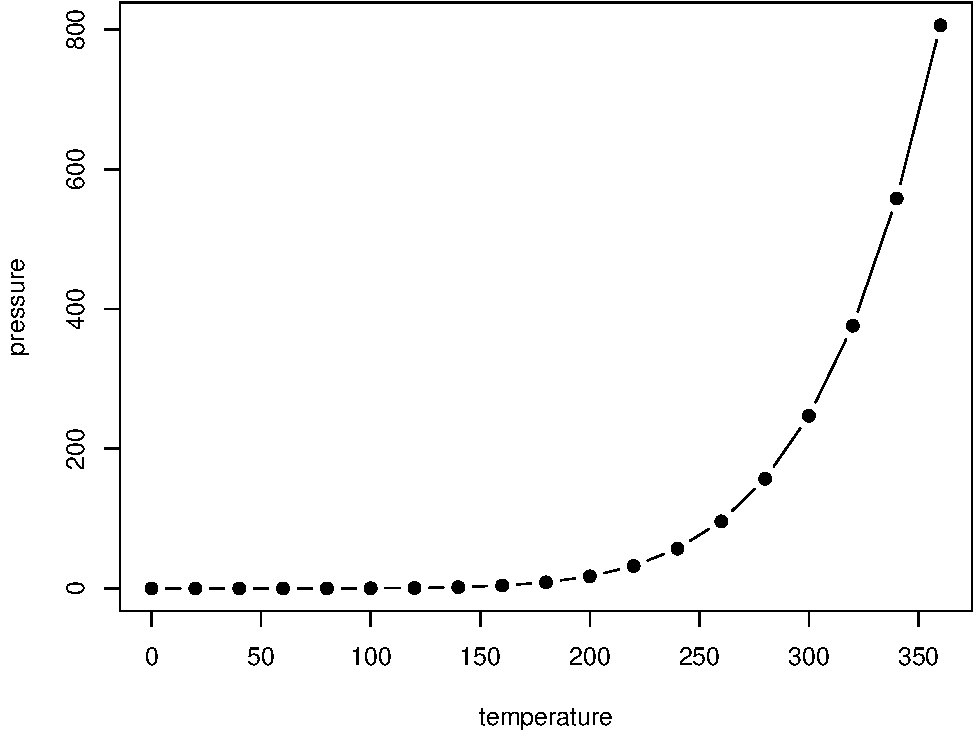
\includegraphics[width=0.6\linewidth]{predissertation_files/figure-latex/nice-fig-1} 

}

\caption{Here is a nice figure!}\label{fig:nice-fig}
\end{figure}

Reference a figure by its code chunk label with the \texttt{fig:}
prefix, e.g., see Figure \ref{fig:nice-fig}.

\hypertarget{tables}{%
\section{Tables}\label{tables}}

The easiest way to create a table is to use Excel to input the
information for your table and save it as a CSV file. Then you can read
in the CSV file, and use the \texttt{kable()} function from
\textbf{knitr} to style the table.

\begin{table}

\caption{\label{tab:nice-tab}2017 Ticket Sales and Operating Revenue for the University of Minnesota Women's Athletic Teams}
\centering
\begin{tabular}[t]{lrr}
\toprule
Sport & Ticket Sales & Total Operating Revenue\\
\midrule
Basketball & 252009 & 873843\\
Cross Country &  & \\
Golf &  & 45197\\
Gymnastics & 38287 & 58288\\
Hockey & 110926 & 389769\\
\addlinespace
Rowing &  & 45454\\
Soccer & 14868 & 33374\\
Softball & 42074 & 98003\\
Swimming \& Diving &  & 74894\\
Tennis &  & 11392\\
\addlinespace
Track and Field &  & 24101\\
Volleyball & 337492 & 485157\\
\bottomrule
\end{tabular}
\end{table}

Further table styling can be carried out via the \textbf{kableExtra}
package; see
\url{https://haozhu233.github.io/kableExtra/awesome_table_in_pdf.pdf}.
You can also reference tables generated from \texttt{knitr::kable()},
e.g., see Table \ref{tab:nice-tab}.

\clearpage

\hypertarget{results}{%
\chapter{Results}\label{results}}

This chapter includes your analyses and results. It should include:

\begin{itemize}
\tightlist
\item
  General data analysis and results
\item
  Data results specific to each hypothesis are presented
\item
  Chapter review
\end{itemize}

Here is a figure of Goldy.

\begin{Shaded}
\begin{Highlighting}[]
\KeywordTok{include_graphics}\NormalTok{(}\DataTypeTok{path =} \StringTok{"figures/goldy.png"}\NormalTok{)}
\end{Highlighting}
\end{Shaded}

\begin{figure}[H]

\includegraphics[width=1.39in]{figures/goldy} \caption{Goldy still rendered as a pencil drawing. This time we overrode the float using the 'H' option.}\label{fig:goldy2}
\end{figure}

You can write citations, too. For example, we are using the
\textbf{bookdown} package \citep{R-bookdown} in this sample book, which
was built on top of R Markdown and \textbf{knitr} \citep{xie2015}.

\clearpage

\hypertarget{discussion}{%
\chapter{Discussion}\label{discussion}}

Summarize the entire project including what hypothesis/questions were
investigated, why they were investigated, how they were investigated,
the major findings, and your conclusions.

\begin{enumerate}
\def\labelenumi{\arabic{enumi}.}
\tightlist
\item
  Discuss the findings and the hypothesis in a holistic and integrated
  fashion.
\item
  Explain any extraneous factors that may have led to the results you
  obtained.
\item
  Discuss the practical and theoretical implications of your findings
  and precisely how your research supports each implication.
\item
  State the conclusions to be drawn from your entire study (including
  review of the literature and empirical findings; i.e., integrate
  everything).
\item
  Discuss suggestion for future research, next stages of research, what
  others might do to follow up on your study.
\end{enumerate}

\clearpage

\bibliography{bib/book.bib,bib/packages.bib}


\end{document}
